\documentclass[a4paper]{article}

\usepackage[english]{babel}
\usepackage[utf8x]{inputenc}
\usepackage{amsmath}
\usepackage{graphicx}
\usepackage{color}
\usepackage{listings}
\usepackage{hyperref}

\title{Report - HMM tutorial}
\author{Soufian SALIM}

\lstset{ %
language=R,                % choose the language of the code
basicstyle=\footnotesize,       % the size of the fonts that are used for the code
numbers=left,                   % where to put the line-numbers
numberstyle=\footnotesize,      % the size of the fonts that are used for the line-numbers
stepnumber=1,                   % the step between two line-numbers. If it is 1 each line will be numbered
numbersep=5pt,                  % how far the line-numbers are from the code
backgroundcolor=\color{white},  % choose the background color. You must add \usepackage{color}
showspaces=false,               % show spaces adding particular underscores
showstringspaces=false,         % underline spaces within strings
showtabs=false,                 % show tabs within strings adding particular underscores
frame=single,           % adds a frame around the code
tabsize=2,          % sets default tabsize to 2 spaces
captionpos=b,           % sets the caption-position to bottom
breaklines=true,        % sets automatic line breaking
breakatwhitespace=false,    % sets if automatic breaks should only happen at whitespace
escapeinside={\%*}{*)}          % if you want to add a comment within your code
}

\begin{document}
\maketitle

\begin{abstract}
Report on the October 9 tutorial course on R's HMM module.

\end{abstract}

\section{Introduction}

From the tutorial's PDF:

\begin{quotation}

We will use from now the HMM package which is available from the CRAN repository
available
(http://cran.rstudio.com/).
It contains the following functions:

\begin{itemize}

\item backward
\item baumWelch
\item dishonestCasino
\item forward
\item initHMM
\item posterior
\item simHMM
\item viterbi
\item viterbiTraining

\end{itemize}

The goal with this exercise is to verify some of the functions that are available, also to let you
understand how all the pieces are working together.

\end{quotation}

\section{Functions}

\subsection{HMMs\_source}

\subsubsection{Description}

Builds two HMMs, using initHMM; the states are “s1” and “s2”, and the symbols “a”, “b”, and “c”.

\subsubsection{Code}

\begin{lstlisting}
HMMs_source <- function() {
  states <- c("s1", "s2")
  obs <- c("a", "b", "c")
  
  P1_source <- c(1, 0)
  A1_source <- matrix(c(0.1,0.9,0.6,0.4), nrow=2, ncol=2, byrow=T)
  B1_source <- matrix(c(0.1,0.3,0.6,0.4,0.2,0.4), nrow=2, ncol=3, byrow=T)
  
  lambda1_source <- initHMM(states, obs, P1_source, A1_source, B1_source)
  
  P2_source <- c(1, 0)
  A2_source <- matrix(c(0.4,0.6,0.8,0.2), nrow=2, ncol=2, byrow=T)
  B2_source <- matrix(c(0.5,0.4,0.1,0.2,0.1,0.7), nrow=2, ncol=3, byrow=T)
  
  lambda2_source <- initHMM(states, obs, P2_source, A2_source, B2_source)
  
  return(list(m1 = lambda1_source, m2 = lambda2_source))
}
\end{lstlisting}

\subsubsection{Results}

\begin{quotation}
\textbf{Call this function, and check the values of source1\_2 <- HMMs\_source()}
\end{quotation}

HMMs\_source() correctly returns two HMMs:

\begin{lstlisting}
$m1
$m1$States
[1] "s1" "s2"

$m1$Symbols
[1] "a" "b" "c"

$m1$startProbs
s1 s2 
 1  0 

$m1$transProbs
    to
from  s1  s2
  s1 0.1 0.9
  s2 0.6 0.4

$m1$emissionProbs
      symbols
states   a   b   c
    s1 0.1 0.3 0.6
    s2 0.4 0.2 0.4


$m2
$m2$States
[1] "s1" "s2"

$m2$Symbols
[1] "a" "b" "c"

$m2$startProbs
s1 s2 
 1  0 

$m2$transProbs
    to
from  s1  s2
  s1 0.4 0.6
  s2 0.8 0.2

$m2$emissionProbs
      symbols
states   a   b   c
    s1 0.5 0.4 0.1
    s2 0.2 0.1 0.7
\end{lstlisting}

\subsection{HMM\_simu}

\subsubsection{Description}

Returns a list of two elements: obs1 and obs2, each of them being a sequence of symbols produced using simHMM.

\subsubsection{Code}

\begin{lstlisting}
HMM_simu <- function(hmm1, hmm2, T = 10){
  return(list(obs1 = simHMM(hmm1, T)$observation, obs2 = simHMM(hmm2, T)$observation))
}
\end{lstlisting}

\subsubsection{Results}

\begin{quotation}
\textbf{Call this function, and check the values of train1\_2 <- HMM\_simu(source1\_2$m1, source1\_2$m2, 1000)}
\end{quotation}

The function returns a series of observations. The possible symbols match those of the HMM defined in HMMs\_source():

\begin{lstlisting}
$obs1
   [1] "c" "b" "b" "a" "b" "a" "b" "c" "b" "c" "b" "c" "c" "a" "c" "a" "a" "b" "c" "b" "a" "c" "a" "c" "c" "c" "a" "a" "a" "b" "a" "c" "c" "a" "a" "c" "c" "b" "c" "c" "c" "a" "c" "c" "c" "c" "a" "c" "a" "c" "b" "c"
 (...)
 [989] "c" "a" "b" "c" "c" "a" "a" "c" "c" "c" "b" "c"

$obs2
   [1] "a" "c" "a" "a" "c" "a" "a" "b" "a" "a" "a" "a" "a" "c" "c" "a" "b" "b" "c" "b" "c" "a" "a" "c" "a" "c" "a" "c" "a" "a" "c" "a" "a" "a" "c" "c" "c" "b" "c" "a" "c" "a" "b" "c" "a" "c" "b" "c" "b" "c" "a" "b"
 (...)
 [989] "a" "a" "c" "c" "b" "c" "a" "a" "a" "a" "a" "c"
\end{lstlisting}

\subsection{logLikelihood}

\subsubsection{Description}

Applies the forward algorithm and then ends with the computation of the likelihood of the observation sequence.

\subsubsection{Code}

\begin{lstlisting}
logLikelihood <- function(hmm, obs){
  fwd <- forward(hmm, obs)
  
  loglike = fwd[1, length(obs)]
  
  for(i in 2:length(hmm$States)){
    t = fwd[i, length(obs)]
    
    if (t > - Inf){
      loglike = t + log(1+exp(loglike-t))
    }
  }
  
  return(loglike)
}
\end{lstlisting}

\subsubsection{Results}

\begin{quotation}
\textbf{Calculate and display the four log-likelihoods P(O1|lambda1), P(O1|lambda2), P(O2|lambda1) and P(O2|lambda2)}
\end{quotation}

\begin{lstlisting}
P(O1|lambda1) =  -51.71073 
P(O1|lambda2) =  -60.70799 
P(O2|lambda1) =  -51.70681 
P(O2|lambda2) =  -57.3821 
\end{lstlisting}

\subsection{HMM\_new}

\subsubsection{Description}

Initializes and returns two new models m1 and m2 with initHMM.

\subsubsection{Code}

\begin{lstlisting}
HMM_new <- function(){
  states <- c("s1","s2")
  obs <- c("a","b","c")
  
  P1 <-c(1,0)
  A1 <- matrix(c(0.8,0.2,0.5,0.5), nrow=2, ncol=2, byrow=T)
  B1 <- matrix(c(0.3,0.4,0.3,0.1,0.8,0.1), nrow=2, ncol=3, byrow=T)
  
  M1 <- initHMM(states, obs, P1, A1, B1)
  M2 <- M1
  
  return(list(m1 = M1, m2 = M2))
}
\end{lstlisting}

\subsection{Check\_likelihood\_BW}

\subsubsection{Description}

Uses the Baum-Welch algorithm and train one HMM, given a sequence of observations, for 10 iterations, and prints the log-likelihood.

\subsubsection{Code}

\begin{lstlisting}
checkLikelihoodBW <- function(hmm, obs){
  hmm_new <- list(hmm=hmm, difference=0)
  
  for(i in 1:10){
    hmm_new <- baumWelch(hmm_new$hmm, obs, 1)
    cat("Likelihood after iteration", i, ": ", logLikelihood(hmm_new$hmm, obs), "\n")
  }
  
  return(hmm_new)
}
\end{lstlisting}

\subsubsection{Results}

\begin{quotation}
\textbf{At each iteration, print the log-likelihood, check that it increases for each iteration. If not, something is wrong in your functions.}
\end{quotation}

The log-likelihood correctly increases at each iteration:

\begin{lstlisting}
Likelihood after iteration 1 :   -104.5332 
Likelihood after iteration 2 :   -104.5329 
Likelihood after iteration 3 :   -104.5326 
Likelihood after iteration 4 :   -104.5322 
Likelihood after iteration 5 :   -104.5319 
Likelihood after iteration 6 :   -104.5317 
Likelihood after iteration 7 :   -104.5314 
Likelihood after iteration 8 :   -104.5312 
Likelihood after iteration 9 :   -104.531 
Likelihood after iteration 10 :  -104.5308 

(...)
\end{lstlisting}

\subsection{train\_BW}

\subsubsection{Description}

Trains two models from their respective training sequence and returns a list of the two HMMs: m1 and m2.

\subsubsection{Code}

\begin{lstlisting}
train_BW <- function(training, N = 10) {
  hmms <- HMM_new()
  
  hmm1 <- baumWelch(hmms$m1,
                    training$obs1,
                    N)

  hmm2 <- baumWelch(hmms$m2,
                    training$obs2,
                    N)
  
  return (list(m1 = hmm1$hmm,
               m2 = hmm2$hmm))
}
\end{lstlisting}

\subsubsection{Results}

\begin{quotation}
\textbf{Compare the original source models with the corresponding trained versions.}
\end{quotation}

\textbf{Common values:}

\begin{lstlisting}
$States
[1] "s1" "s2"

$Symbols
[1] "a" "b" "c"

$startProbs
s1 s2 
 1  0 
\end{lstlisting}

\textbf{Original source model:}

\begin{lstlisting}
$transProbs
    to
from  s1  s2
  s1 0.1 0.9
  s2 0.6 0.4

$emissionProbs
      symbols
states   a   b   c
    s1 0.1 0.3 0.6
    s2 0.4 0.2 0.4
\end{lstlisting}

\textbf{Trained model (10 iterations):}

\begin{lstlisting}
$transProbs
    to
from        s1        s2
  s1 0.5639968 0.4360032
  s2 0.3743099 0.6256901

$emissionProbs
      symbols
states         a          b          c
    s1 0.1641866 0.08025629 0.75555710
    s2 0.4012511 0.53199452 0.06675439
\end{lstlisting}

\begin{quotation}
\textbf{Discuss and explain your results.}
\end{quotation}

Transition and emission matrices have changed after training to adjust better to the observed data. Given the set of observations, the Baum-Welch algorithm adjusted the probabilities at each iteration to converge towards the maximum likelihood estimate of the HMM parameters.

\subsection{classify}

\subsubsection{Description}
Displays the confusion matrix and returns the recognition rate, when using source1\_2 to generate N test samples of length T of each source and lambda1\_2 as classifiers.

\subsubsection{Code}

\begin{lstlisting}
classify <- function(source1_2, model1_2, T = 10, N = 1) {
  true_pos = false_pos = true_neg = false_neg = 0
  
  for (i in 1:(N / 2)) {
    test1_2 <- HMM_simu(source1_2$m1, source1_2$m2, T)
    
    r <- list(
      o1m1 = logLikelihood(model1_2$m1, test1_2$obs1),
      o1m2 = logLikelihood(model1_2$m2, test1_2$obs1),
      o2m1 = logLikelihood(model1_2$m1, test1_2$obs2),
      o2m2 = logLikelihood(model1_2$m2, test1_2$obs2)
    )
    
    if (r$o1m1 > r$o1m2)
      true_pos = true_pos + 1
    else
      false_neg = false_neg + 1
    if (r$o2m2 > r$o2m1)
      true_neg = true_neg + 1
    else
      false_pos = false_pos + 1
  }
  
  print(
    matrix(
      c(true_pos, false_neg, false_pos, true_neg),
      ncol = 2,
      nrow = 2,
      byrow = TRUE,
      dimnames = list(
        c("is true", "is false"), 
        c("found true", "found false")
      )
    )
  )
  
  return (true_pos + true_neg) / N
}
\end{lstlisting}

\subsubsection{Results}

\textbf{Confusion matrix:}

\hspace{20mm}

\begin{tabular}{ c | c | c }
  & Found True & Found False \\
  \hline
  Is True & 316 & 184 \\
  \hline
  Is False & 73 & 427 \\
\end{tabular}

\hspace{20mm}

\begin{lstlisting}
         found true found false
is true         316         184
is false         73         427
\end{lstlisting}

\textbf{Recognition rate:}

\hspace{10mm}

743 recognized out of 1000 (74.3%)

\hspace{10mm}

\subsection{Plot\_Reco}

\subsubsection{Description}
Computes and plot the curve which displays the evolution of the recognition rate according to the length of the observed test sequences. Scan a range of 10 values up to Tmax.
\subsubsection{Code}

\begin{lstlisting}
Plot_Reco <- function(source1_2, model1_2, Tmax = 100, N = 1) {
  reco_rate <- NULL
  samples_size <- 1:10 * (Tmax/ 10)
  
  for (i in 1:10 * (Tmax/ 10)) {
    reco_rate <- c(reco_rate, (classify(source1_2,
                               model1_2,
                               i,
                               N)) / N)
  }
  
  plot(samples_size, reco_rate, type = "l", col = "blue", xlab = "Samples size", ylab = "Recognition rate")
}
\end{lstlisting}

\subsubsection{Results}

\begin{figure}[ht!]
\centering
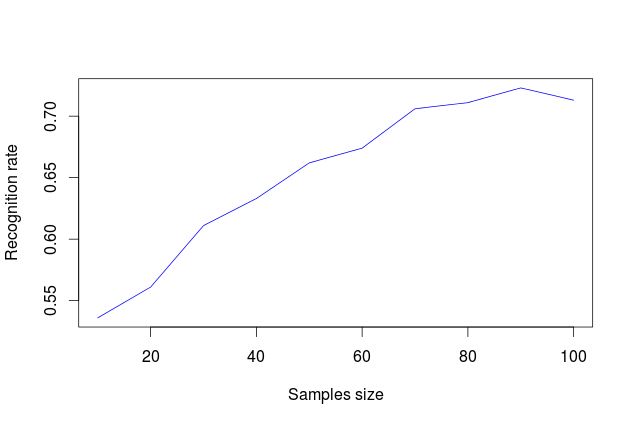
\includegraphics[width=90mm]{recograph.png}
\caption{Recognition rate by sample size}
\label{overflow}
\end{figure}

\subsection{Compare\_States}

\subsubsection{Description}
Compares the true sequence of states followed by a model and the one obtained from the Viterbi algorithm.

\subsubsection{Code}

\begin{lstlisting}
Compare_States <- function(hmm, obs, states) {
  return(
    1 - length(
      Filter(identity, states != viterbi(hmm, obs))
    )
    / length(states)
  )
}
\end{lstlisting}

\subsubsection{Results}

\begin{quotation}
\textbf{Simulate a sequence (states and observations), use the observation to look for the most
probable path for this sequence using the source model. What is the percentage of correct assignments??}
\end{quotation}

\begin{lstlisting}
Correct proportion for M1 on O1 compared to Viterbi:  0.51 
Correct proportion for M2 on O2 compared to Viterbi:  0.42 
\end{lstlisting}

\begin{quotation}
\textbf{Would you consider that useful performance?}
\end{quotation}

A result graviting around 50\% is hardly useful.

\begin{quotation}
\textbf{Perform the same experiment but used the trained model instead of source model to do the alignment.}
\end{quotation}

\begin{lstlisting}
Correct proportion for M1 on O1 compared to Viterbi:   0.57 
Correct proportion for M2 on O2 compared to Viterbi:   0.6 
\end{lstlisting}

We note a significant improvement in results.

\section{Attachments}

The code described in this document can be found here: \url{http://github.com/bolaft/signal_hmm}

\end{document}